\section{Andengradsligninger}

I denne opgave skal vi løse andengradsligninger. For at løse en andengradsligning skal vi bruge følgende theorem

\begin{frm-thm}{Løsning af andengradsligning}\thlabel{anden}

Hvis vi har en andengradsligning på følgende form \hspace*{2cm} $ax^2 + bx + c$

Hvor diskriminanten D beregnes ved \hspace*{4.2cm} $D = b^2 -4ac$

Har andengradsligningen følgende løsninger

\vspace*{4mm}

Hvis $D < 0$ findes der ingen løsninger

Hvis $D = 0$ findes der en løsning \hspace*{4.7cm} $x = \cfrac{-b}{2a}$

Hvis $D > 0$ findes der 2 løsninger \hspace*{4.6cm} $x_1 = \cfrac{-b + \sqrt{D}}{2a}, \hspace*{4mm} x_2 = \cfrac{-b - \sqrt{D}}{2a}$

\end{frm-thm}

\subsection{Opgave}
Løs andengradsligningen $2x^2 + 4x + 2 = 0$

Vi starter med at aflæse a,b og c fra andengradsligningen. Vi ved at a står foran $x^2$, b står foran $x$ og c står for sig selv. Derfor er 
\begin{align*}
a &= 2\\
b &= 4\\
c &= 2
\end{align*}

Når vi har aflæst a, b og c ud fra andengradsligningen beregner vi diskriminanten D. Diskriminanten fortæller os om andengradsligningen har 0, 1 eller 2 løsninger. Vi beregner nu diskriminanten D

\begin{align*}
D = b^2 - 4ac = 4^2 - 4 \cdot 2 \cdot 2 = 16 - 16 = 0
\end{align*}

Da diskriminanten er 0 fortæller Theorem \ref{anden} os at andengradsligningen har 1 løsning. Vi beregner nu løsningen til andengradsligningen

\begin{align*}
x = \frac{-b}{2a} = \frac{-4}{2\cdot 2} = \frac{-4}{4} = -1
\end{align*}

Løsningen til andengradsligningen er dermed $x = -1$. Ligesom i afsnittet om simple ligninger kan vi tjekke om vi har fået det korrekte resultat ved at indsætte $x=-1$ på x's plads i andengradsligningen og se om begge sider af lighedstegnet er ens.

\begin{align*}
2x^2 +4x + 2 &= 0\\
\Updownarrow \hspace*{36mm} &\\
2\cdot (-1)^2 + 4\cdot (-1) + 2 &= 0 && \text{Indsætter} \hspace{1mm} x=-1 \hspace*{1mm} \text{på x's plads}\\
\Updownarrow \hspace*{36mm} &\\
2\cdot 1 -4 + 2 &= 0\\
\Updownarrow \hspace*{36mm} &\\
-2 + 2 &= 0\\
\Updownarrow \hspace*{36mm} &\\
0 &= 0
\end{align*}

Da begge sider af lighedstegnet er ens har vi altså fundet den korrekte løsning til andengradsligningen. Det er ikke nødvendigt at tjekke om man har fået den rigtige løsning men hvis man er i tvivl kan man lave det samme tjek som vi har gjort ovenfor.

Når vi i denne opgave løser andengradsligning  $2x^2 +4x + 2 = 0$ finder vi de x værdier hvor vores parabel $f(x) = 2x^2 +4x + 2$ rammer/skærer x-aksen. I vores tilfælde rammer/skærer vores parabel x aksen når $x = -1$. Nedenfor kan i se dette ilustreret grafisk ved at indtegne parablen $f(x) = 2x^2 + 4x + 2$ i geogebra. Det eneste sted parablen rører x-aksen er præcis når $x=-1$.

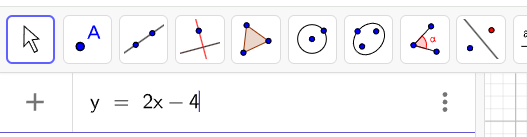
\includegraphics[scale=0.7]{img_1}